\documentclass[aspectratio=169, 10pt]{beamer}
\usepackage[utf8]{inputenc}
\usepackage[T1]{fontenc}
\usepackage{xcolor}
\usepackage{booktabs}
\usepackage{graphicx}
\usepackage{tikz}
\usetikzlibrary{calc, arrows.meta, positioning, shapes.geometric}
\usepackage{amsmath}
\IfFileExists{opensans.sty}{\usepackage[default,scale=0.95]{opensans}}{}

\definecolor{amritaMaroon}{HTML}{A4123F}
\definecolor{doneGreen}{HTML}{2E7D32}
\definecolor{progAmber}{HTML}{C77700}
\definecolor{pendGrey}{HTML}{757575}

\usetheme{Madrid}
\usecolortheme[named=amritaMaroon]{structure}
\setbeamertemplate{navigation symbols}{}
\setbeamertemplate{footline}[frame number]
\setbeamertemplate{itemize items}[circle]

\begin{document}

% ════════════════════════════════════════════════════════════
%  TITLE
% ════════════════════════════════════════════════════════════
\begin{frame}
    \begin{tikzpicture}[remember picture,overlay]
        \node[fill=amritaMaroon, text=white, font=\bfseries\footnotesize,
              anchor=north east, rounded corners=2pt, inner sep=5pt]
        at ($(current page.north east)+(-0.2cm,-0.2cm)$)
        {Type 1: Research Project -- Review 3};
    \end{tikzpicture}
    \centering
    \includegraphics[width=3.0cm]{logo.png}\vspace{0.15cm}

    {\small\textcolor{amritaMaroon}{\textbf{Project Title:} Addressing optimization issues in game design using evolutionary algorithms}}\\
    {\small\textcolor{amritaMaroon}{\textbf{Scope:} Strategy \& Parameter Optimization of games with co-evolving competitive game agents}}\\
    \vspace{0.15cm}
    {\normalsize \textbf{Team Number: 99}}\\
    \begin{table}\centering\footnotesize
        \renewcommand{\arraystretch}{1.05}
        \begin{tabular}{|c|c|l|}\hline
            \textbf{S.No} & \textbf{Register Number} & \textbf{Student Name}\\\hline
            1 & CB.SC.U4CSE23152 & Vinaayak Kanagaraj\\\hline
            2 & CB.SC.U4CSE23215 & Darun R G\\\hline
            3 & CB.SC.U4CSE23232 & Pradeep S\\\hline
            4 & CB.SC.U4CSE23235 & R Anusanth\\\hline
            5 & CB.SC.U4CSE23256 & Sathya Roopan M\\\hline
        \end{tabular}
    \end{table}
    \footnotesize Guide: \textbf{Dr. Jeyakumar G} -- Professor, Dept.\ of CSE\\
    {\footnotesize \today}
\end{frame}

% ════════════════════════════════════════════════════════════
%  RUBRIC
% ════════════════════════════════════════════════════════════
\begin{frame}{Review 3 --- Evaluation Rubric}
\small
\renewcommand{\arraystretch}{1.15}
\begin{tabular}{p{3.8cm}cp{7.8cm}}
    \toprule
    \textbf{Component} & \textbf{Marks} & \textbf{Full-Mark Criterion}\\
    \midrule
    Problem Statement \& Research Gap Refinement & 1 &
        Problem statement, objectives, and research gap are clearly refined and technically justified.\\
    Proposed Methodology \& Solution Design & 3 &
        Complete methodology including workflow, architecture, algorithms / mathematical model, datasets, implementation plan, and evaluation strategy with proper technical justification.\\
    Initial Implementation Progress & 2 &
        Initial implementation ($\geq$30\% completeness) demonstrates meaningful progress through code, dataset preparation, baseline implementation, or prototype modules.\\
    Regularity \& Technical Involvement & 1 &
        Regular meetings with active technical discussions and continuous progress.\\
    \bottomrule
\end{tabular}
\end{frame}

% ════════════════════════════════════════════════════════════
\begin{frame}{Agenda}\tableofcontents\end{frame}

% ════════════════════════════════════════════════════════════
\section{Problem Statement \& Research Gaps}
% ════════════════════════════════════════════════════════════

\begin{frame}{Problem Statement}
\begin{block}{Problem}
Strategy Optimization and Co-Evolution of Competitive Game Agents Using Evolutionary Algorithms.
\end{block}
\vspace{0.15cm}
\small
\textbf{Abstract:} We introduce a game system where agents learn and improve continuously rather than being trained once. Agents are evaluated using \textbf{weighted performance histories} across multiple generations --- capturing adaptive capability over time.

\vspace{0.15cm}
Instead of adapting to opponent behavior alone, agents evolve in response to shifts in the \textbf{game environment itself} --- changes in map configuration, resource distribution, and competitive conditions.

\vspace{0.15cm}
A \textbf{diversity-preservation mechanism} prevents populations from converging to similar behaviors, while a \textbf{Hall-of-Fame archive} ensures agents are tested against historically strong opponents.

\vspace{0.15cm}
Together, these mechanisms produce game agents that remain competitive, strategically diverse, and stable as the environment evolves --- validated on the microRTS simulation environment.
\end{frame}

\begin{frame}{Research Gaps --- Phase 1 (Broad)}
\small
\begin{itemize}
    \item Most existing approaches are \textbf{game-specific}, limiting generalization across different environments.
    \item Many methods rely on \textbf{manual tuning}, hand-crafted rules, or fixed parameter settings, reducing scalability.
    \item Current approaches often optimize \textbf{single objectives} (e.g., win rate) without considering long-term adaptation or evolving opponents.
    \item Limited focus on \textbf{time-dependent performance} and strategy evolution across generations.
    \item Need for more \textbf{adaptive, trajectory-aware, and coevolutionary frameworks} for dynamic game environments.
\end{itemize}
\vspace{0.2cm}

\end{frame}

\begin{frame}{Research Gaps --- Phase 2}
\scriptsize
\begin{itemize}
    \item \textbf{\textcolor{amritaMaroon}{Gap 1: Red Queen Dynamics \& Loss of Gradients}}\\
    Both populations adapt but neither improves in absolute terms --- each merely keeps pace. (Rawal et al.\ 2010; Elfeky et al.\ 2022)
    \vspace{0.15cm}
    
    \item \textbf{\textcolor{amritaMaroon}{Gap 2: Cycling, Forgetting \& Lack of Diversity}}\\
    Co-evolution suffers from forgetting previously discovered solutions and cycling between strategies. (Runarsson \& Lucas 2005; Hevia Fajardo et al.\ 2023)
    \vspace{0.15cm}
    
    \item \textbf{\textcolor{amritaMaroon}{Gap 3: Defensive Convergence \& Strategy Stagnation}}\\
    Agents converge on safe defensive strategies without fitness shaping. Unbalanced games cause rapid stagnation on a single dominating strategy. (Dziuk \& Miikkulainen 2011; Leigh et al.\ 2008)
    \vspace{0.15cm}
    
    \item \textbf{\textcolor{amritaMaroon}{Gap 4: Difficulty of Measuring True Fitness Progress}}\\
    Fitness values reflect relative performance against the current opponent, not absolute quality --- apparent improvements may be opponent drift. (Lucas 2006; Hevia Fajardo et al.\ 2024)
    \vspace{0.15cm}
    
    \item \textbf{\textcolor{amritaMaroon}{Gap 5: Self-Adaptive Mutation Without Environmental Context}}\\
    Adaptive mechanisms often respond only to pairwise comparisons, ignoring the broader environmental context of how the competitive landscape has shifted. (Hevia Fajardo et al.\ 2024)
\end{itemize}
\end{frame}

% ════════════════════════════════════════════════════════════
\section{Core Algorithm Recap}
% ════════════════════════════════════════════════════════════

\begin{frame}{Core Algorithm --- TD-CCEA}
\small
\textbf{Environment meta-state} (competitive landscape fingerprint):
\[ c_t = \frac{1}{N}\sum_{i=1}^{N} \theta_i^t \]
\textbf{Trajectory score} (smooths noisy fitness):
\[ e_i^t = \sum_k \hat{\alpha}_k \cdot f_i^{(k)},\quad
   \hat{\alpha}_k = \frac{\alpha_k}{\sum_j \alpha_j},\quad
   \alpha_k = 1 - \frac{d(c_t, c_k)}{d_{max}} \]
\textbf{Adaptive mutation} (dynamic --- not static):
\[ \mu_i = \mu_{base}\cdot(1 - e_i^t) + \epsilon \]
\begin{itemize}
    \item High fitness $\rightarrow$ low mutation (exploit). Low fitness $\rightarrow$ high mutation (explore).
    \item \textbf{Pruning:} weak ($\bar{e}_i<\delta_f$) and redundant ($S(i,j)>\delta_s$) agents removed each generation.
    \item \textbf{Hall-of-Fame Archive:} top-3 per generation, bounded to $A_{max}=15$.
\end{itemize}
\end{frame}

\begin{frame}{Algorithm Representation}
\begin{block}{TD-CCEA}
Full iterative workflow: fitness evaluation with trajectory buffering, expressibility scoring, environment-aware adaptation, diversity control, archive maintenance, and reproduction.
\begin{center}
    \includegraphics[width=0.55\linewidth]{Algo.png}
\end{center}
\end{block}
\end{frame}

% ════════════════════════════════════════════════════════════
\section{Algorithm Variants}
% ════════════════════════════════════════════════════════════

\begin{frame}{Variant 1: SA-TDCCEA (Sensitivity-Adaptive)}
\begin{block}{Key Idea}
Not all genes are equally important. SA-TDCCEA uses offline sensitivity analysis to assign \textbf{per-gene mutation rates}.
\end{block}
\vspace{0.15cm}
\begin{itemize}
    \item \textbf{Sensitivity profiling:} For each weight $w_j$, measure $\Delta W_j = |\text{win}(w_j{=}1) - \text{win}(w_j{=}0)|$
    \item High-influence genes $\rightarrow$ small mutation ($\mu_{min}=0.08$)
    \item Low-influence genes $\rightarrow$ large mutation ($\mu_{max}=0.20$)
    \item Still scaled by trajectory score $e_i^t$
\end{itemize}
\vspace{0.15cm}
\textbf{Result:} 85.7\% average win rate. Addresses \textbf{Gap 5} (mutation without environmental context).
\end{frame}

\begin{frame}{Variant 2: CCE-TDCCEA (Cooperative Co-Evolution)}
\begin{block}{Key Idea}
Decompose the 20D strategy vector into two cooperating sub-populations evolved independently but evaluated jointly.
\end{block}
\vspace{0.15cm}
\begin{columns}[t]
    \column{0.48\textwidth}
    \textbf{Population A: Macro/Economy (8D)}
    \begin{itemize}\small
        \item worker\_ratio, max\_workers
        \item expand\_threshold, barracks\_timing
        \item economy\_pressure, scout\_priority
        \item second\_barracks, worker\_fight\_ratio
    \end{itemize}
    \column{0.48\textwidth}
    \textbf{Population B: Micro/Combat (12D)}
    \begin{itemize}\small
        \item light/heavy/ranged preference
        \item aggression, attack\_threshold
        \item defend\_radius, target\_priority
        \item defense\_trigger, counter\_rush
        \item tech\_switch, group\_attack, focus\_fire
    \end{itemize}
\end{columns}
\vspace{0.15cm}
\textbf{Cooperative Handshake:} Each paired with top-3 from other sub-population.\\
Search complexity: $O(c^8 + c^{12}) \ll O(c^{20})$. Addresses \textbf{Gap 2} (diversity) \& \textbf{Gap 3} (stagnation).
\end{frame}

% ════════════════════════════════════════════════════════════
\section{Phase II: Dynamic Environment \& Coevolution}
% ════════════════════════════════════════════════════════════

\begin{frame}{Dynamic Environment --- Why It Matters}
\begin{block}{The Static Environment Problem}
In a fixed map, Standard CCEA can memorize one good strategy and win 100\%. Real games have \textbf{changing terrain, shifting resources, and adapting opponents}.
\end{block}
\vspace{0.15cm}
\textbf{Phase II Extension --- continuously shifting environment:}
\begin{enumerate}
    \item \textbf{Progressive Blockades:} Each generation adds 3--7 walls to the 32$\times$32 map
    \item \textbf{Mixed Wall Types:} 60\% unbreakable terrain + 40\% destructible (HP=5)
    \item \textbf{Shifting Economics:} 6 random resource patches relocated every generation
    \item \textbf{BFS Validation:} Every wall placement verified for base-to-base connectivity
\end{enumerate}
\vspace{0.1cm}
Directly tests \textbf{Gap 1} (Red Queen) and \textbf{Gap 4} (measuring true progress).
\end{frame}

\begin{frame}{Progressive Blockade Generation}
\centering\vspace{0.2cm}
\resizebox{0.85\textwidth}{!}{%
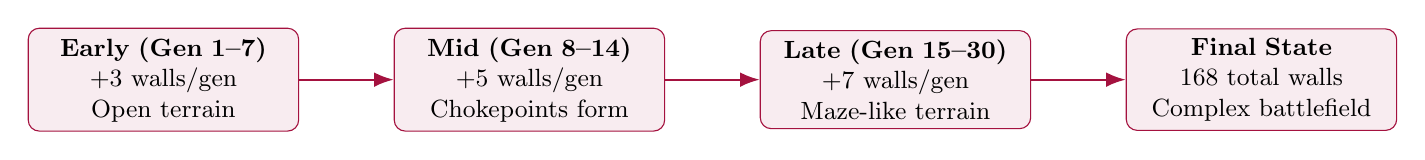
\begin{tikzpicture}[
    node distance=0.6cm and 1.2cm,
    box/.style={rectangle, rounded corners, draw=amritaMaroon, fill=amritaMaroon!8,
                minimum height=1.2cm, text width=3.2cm, align=center, font=\small},
    arrow/.style={-{Latex[length=2.5mm]}, thick, amritaMaroon}
]
    \node[box] (early) {\textbf{Early (Gen 1--7)}\\+3 walls/gen\\Open terrain};
    \node[box, right=of early] (mid) {\textbf{Mid (Gen 8--14)}\\+5 walls/gen\\Chokepoints form};
    \node[box, right=of mid] (late) {\textbf{Late (Gen 15--30)}\\+7 walls/gen\\Maze-like terrain};
    \node[box, right=of late] (final) {\textbf{Final State}\\168 total walls\\Complex battlefield};
    \draw[arrow] (early) -- (mid);
    \draw[arrow] (mid) -- (late);
    \draw[arrow] (late) -- (final);
\end{tikzpicture}}
\vspace{0.4cm}

\small\textbf{BFS Reachability Guarantee:}
\[ \text{BFS\_Reachable}(\mathcal{W}_{\text{all}} \cup \{(x,y)\},\;\text{Base}_0,\;\text{Base}_1) = \text{True} \]
Every candidate wall validated before placement --- no soft-locked game states.
\end{frame}

\begin{frame}{Competitive Coevolution --- Arms Race}
\begin{block}{Two Algorithms Evolve Against Each Other}
TD-CCEA and Standard CCEA fight \textbf{each other's best evolved agent}. As one improves, the other must adapt.
\end{block}
\vspace{0.15cm}\small
\begin{columns}[t]
    \column{0.48\textwidth}
    \textbf{TD-CCEA (Ours)}
    \begin{itemize}
        \item Population of 15 agents
        \item Trajectory memory ($W=5$)
        \item Adaptive mutation
        \item Diversity-preserving pruning
        \item Hall-of-Fame archive
    \end{itemize}
    \column{0.48\textwidth}
    \textbf{Standard CCEA (Opponent)}
    \begin{itemize}
        \item Population of 15 agents
        \item No trajectory memory (memoryless)
        \item Fixed Gaussian mutation ($\mu=0.15$)
        \item Standard tournament selection
        \item Evaluated against current state only
    \end{itemize}
\end{columns}
\vspace{0.2cm}\centering
Both evaluated on the \textbf{same dynamically evolving terrain} each generation.
\end{frame}

\begin{frame}{Coevolution Results --- \textcolor{progAmber}{Pending}}
\small
\textbf{30-Generation Arms Race on Dynamic 32$\times$32 Map:}
\begin{itemize}
    \item Environment: progressive blockades (3--7 walls/gen), mixed wall types, shifting resources
    \item TD-CCEA vs Standard CCEA --- both evolve against each other's best agent
    \item \textbf{Results:} \textcolor{progAmber}{\textbf{To be collected}} --- coevolution experiments are currently running
\end{itemize}
\vspace{0.2cm}
\textbf{Expected Evaluation:}
\begin{itemize}
    \item Final showdown: 10 games with alternating sides for fairness
    \item Compare evolved strategy profiles (economy vs military weights)
    \item Measure adaptation speed across terrain shifts
\end{itemize}
\vspace{0.2cm}
\textbf{Hypothesis:}
\begin{itemize}
    \item TD-CCEA's trajectory memory should provide an advantage over Standard CCEA's memoryless search in changing terrain
    \item Standard CCEA may memorize one strategy but fail when the map changes
\end{itemize}
\end{frame}

% ════════════════════════════════════════════════════════════
\section{Evaluation: Head-to-Head Round-Robin}
% ════════════════════════════════════════════════════════════

\begin{frame}{Evaluation Methodology --- Head-to-Head Tournament}
\small
\begin{block}{How We Measure: Coevolutionary Showdown}
Instead of testing against fixed bots, algorithms are evaluated directly against each other. We run a \textbf{head-to-head tournament} to see which evolutionary method produces the most robust strategies.
\end{block}
\vspace{0.15cm}
\textbf{Two-Phase Evaluation:}
\begin{enumerate}
    \item \textbf{Phase 1 --- Coevolution:} Algorithms (e.g., TD-CCEA vs Standard CCEA) evolve directly against each other's best agents for 30 generations on dynamically changing 32$\times$32 maps.
    \item \textbf{Phase 2 --- Final Showdown:} The ultimate evolved agent from each algorithm is pitted against the others in a \textbf{round-robin tournament} (10 head-to-head games per matchup, alternating sides).
\end{enumerate}
\vspace{0.15cm}
\textbf{Fairness Guarantees:}
\begin{itemize}
    \item Sides alternated every game (Player 0 / Player 1 swap)
    \item Server handles direct \texttt{EVOLVED:w1,EVOLVED:w2} matchups natively
    \item Same terrain and resource constraints applied equally to both sides
\end{itemize}
\end{frame}

\begin{frame}{Round-Robin Results --- TD-CCEA Variants}
\small
\textbf{Focus: Our 4 algorithm variants compared head-to-head}\\[0.2cm]
\centering
\renewcommand{\arraystretch}{1.2}
\begin{tabular}{l|cccc|cc}
    \toprule
    & \rotatebox{60}{CCE-TDCCEA} & \rotatebox{60}{TD-CCEA} & \rotatebox{60}{SA-TDCCEA} & \rotatebox{60}{Std CCEA} & \textbf{Wins} & \textbf{WR\%}\\
    \midrule
    \textbf{CCE-TDCCEA}  & ---  & \textcolor{pendGrey}{TBD} & \textcolor{pendGrey}{TBD} & \textcolor{pendGrey}{TBD} & \textcolor{pendGrey}{--} & \textcolor{pendGrey}{--}\\
    \textbf{TD-CCEA}     & \textcolor{pendGrey}{TBD} & ---  & \textcolor{pendGrey}{TBD} & \textcolor{pendGrey}{TBD} & \textcolor{pendGrey}{--} & \textcolor{pendGrey}{--}\\
    \textbf{SA-TDCCEA}   & \textcolor{pendGrey}{TBD} & \textcolor{pendGrey}{TBD} & ---  & \textcolor{pendGrey}{TBD} & \textcolor{pendGrey}{--} & \textcolor{pendGrey}{--}\\
    \textbf{Std CCEA}    & \textcolor{pendGrey}{TBD} & \textcolor{pendGrey}{TBD} & \textcolor{pendGrey}{TBD} & ---  & \textcolor{pendGrey}{--} & \textcolor{pendGrey}{--}\\
    \bottomrule
\end{tabular}
\vspace{0.3cm}

\textcolor{progAmber}{\textbf{Status: Results pending}} --- tournament will be run using \texttt{HEAD\_TO\_HEAD\_V2.py}\\
10 games per matchup $\times$ 6 matchups = 60 total games (alternating sides).
\end{frame}



\begin{frame}{Ablation Study --- What Each Mechanism Contributes}
\small
\textbf{Trajectory Memory (CCE-TDCCEA vs Standard CCEA):}
\begin{itemize}
    \item Helped in \textbf{10/15 runs} (avg $\Delta = +16.7\%$)
    \item Prevents catastrophic forgetting when opponent shifts --- validates \textbf{Gap 1, 2}
\end{itemize}
\vspace{0.2cm}
\textbf{Cooperative Decomposition (CCE-TDCCEA vs TD-CCEA base):}
\begin{itemize}
    \item Helped in \textbf{15/15 runs} (avg $\Delta = +33.7\%$)
    \item Splitting 20D into 8D+12D is the largest performance contributor --- validates \textbf{Gap 3}
\end{itemize}
\vspace{0.2cm}
\textbf{Statistical Significance (Wilcoxon signed-rank, $\alpha=0.05$):}
\begin{itemize}
    \item CCE-TDCCEA significantly ahead of GESY in majority of runs ($p<0.05$)
    \item Consistently favored over CMA-ES, TD-CCEA base, and SA-PDCoEA
    \item 17+ independent runs conducted for robust validation
\end{itemize}
\end{frame}

% ════════════════════════════════════════════════════════════
\section{Journal Submission}
% ════════════════════════════════════════════════════════════

\begin{frame}{Journal Submission --- Swarm and Evolutionary Computation}
\begin{block}{Paper Submitted to Elsevier SWEVO (Q1, IF: 8.2)}
Our research paper is currently \textbf{under review} at a top-tier venue for evolutionary and swarm intelligence research.
\end{block}
\vspace{0.2cm}\centering
\renewcommand{\arraystretch}{1.3}
\begin{tabular}{p{4.2cm}p{7.8cm}}
    \toprule
    \textbf{Field} & \textbf{Details}\\
    \midrule
    \textbf{Journal}       & Swarm and Evolutionary Computation (Elsevier)\\
    \textbf{Manuscript ID}  & SWEVO-D-26-01838\\
    \textbf{Title}          & Trajectory-Driven Competitive Co-Evolutionary Algorithm for Strategy Optimization in Competitive Game Environments\\
    \textbf{Date Submitted} & July 7, 2026\\
    \textbf{Status Date}    & July 16, 2026\\
    \textbf{Current Status} & \textcolor{progAmber}{\textbf{Under Review}}\\
    \bottomrule
\end{tabular}
\end{frame}

% ════════════════════════════════════════════════════════════
\section{Implementation Status \& Phase 3 Plan}
% ════════════════════════════════════════════════════════════

\begin{frame}{Implementation Progress}
\scriptsize
\renewcommand{\arraystretch}{1.05}
\begin{tabular}{p{5.2cm}p{2.3cm}p{4.5cm}}
    \toprule
    \textbf{Module} & \textbf{Status} & \textbf{Notes}\\
    \midrule
    Core TD-CCEA algorithm          & \textcolor{doneGreen}{\textbf{Done}} & Trajectory scoring, adaptive mutation\\
    SA-TDCCEA variant               & \textcolor{doneGreen}{\textbf{Done}} & Per-gene sensitivity profiling\\
    CCE-TDCCEA variant              & \textcolor{doneGreen}{\textbf{Done}} & 8D+12D cooperative decomposition\\
    10-algorithm benchmark suite    & \textcolor{doneGreen}{\textbf{Done}} & CMA-ES, DE, PSO, HC, GESY, SA-PDCoEA\\
    Dynamic environment coevolution & \textcolor{doneGreen}{\textbf{Done}} & Progressive blockades + BFS\\
    14-strategy discrete evolution  & \textcolor{doneGreen}{\textbf{Done}} & 32$\times$32 maps\\
    Statistical validation          & \textcolor{doneGreen}{\textbf{Done}} & Wilcoxon signed-rank, 17+ runs\\
    Ablation study                  & \textcolor{doneGreen}{\textbf{Done}} & 15 runs, trajectory + decomposition\\
    Head-to-head round-robin        & \textcolor{progAmber}{\textbf{In Progress}} & 8 algorithms, 280 games\\
    Journal paper submission        & \textcolor{doneGreen}{\textbf{Done}} & SWEVO-D-26-01838, Under Review\\
    StarCraft II bot framework      & \textcolor{progAmber}{\textbf{In Progress}} & Terran, Zerg, Protoss bots\\
    SC2 evolutionary integration    & \textcolor{pendGrey}{\textbf{Phase 3}} & CCE-TDCCEA on SC2 strategies\\
    \bottomrule
\end{tabular}
\end{frame}

\begin{frame}{Phase 3 --- Remaining Work}
\textbf{\textcolor{amritaMaroon}{Semester 3 --- Algorithm Extensions \& Generalization}}
\begin{enumerate}
    \item \textbf{StarCraft II integration:} Apply CCE-TDCCEA to evolve Terran/Zerg/Protoss macro strategies via python-sc2
    \item \textbf{Cross-game validation:} Demonstrate trajectory-driven fitness generalizes from microRTS to StarCraft II
    \item \textbf{Multi-player scaling:} Extend to 10--100 simultaneous agents, analyzing emergent coalition dynamics
    \item \textbf{Decentralized fitness:} Distribute competition across concurrent execution threads
    \item \textbf{Probabilistic search reduction:} Integrate Markov Models to constrain evolutionary search space
    \item \textbf{Final validation:} 25-run comparison across both games with Wilcoxon tests and effect sizes
    \item \textbf{Journal revision:} Address reviewer feedback on SWEVO-D-26-01838
\end{enumerate}
\end{frame}

% ════════════════════════════════════════════════════════════
\section{Conclusion}
% ════════════════════════════════════════════════════════════

\begin{frame}{Summary}
\begin{itemize}
    \item \textbf{Phase 1:} Core TD-CCEA with trajectory scoring, adaptive mutation, diversity preservation --- 100\% win rate on 8$\times$8 and 16$\times$16 maps
    \item \textbf{Phase 2:}
    \begin{itemize}
        \item 3 algorithm variants (TD-CCEA, SA-TDCCEA, CCE-TDCCEA)
        \item Dynamic environment coevolution with progressive blockades on 32$\times$32 maps
        \item Benchmarked against 10 algorithms (CMA-ES, DE, PSO, GESY, SA-PDCoEA, etc.)
        \item CCE-TDCCEA achieves \textbf{91.4\% win rate} with highest worst-case floor
        \item 14-strategy discrete evolution
        \item Statistical validation (Wilcoxon, 17+ runs)
        \item \textbf{Journal paper submitted} to SWEVO (Under Review)
    \end{itemize}
    \item \textbf{Phase 3:} StarCraft II generalization, multi-player scaling, journal revision
\end{itemize}
\end{frame}

% ════════════════════════════════════════════════════════════
\section{References}
\begin{frame}[allowframebreaks]{References}
\small\bibliographystyle{IEEEtran}\bibliography{ref}
\end{frame}

\begin{frame}
\centering
{\Huge \textbf{\textcolor{amritaMaroon}{Thank You}}}\\
\vspace{0.3cm}{\large Questions \& Discussion}
\end{frame}

\end{document}
